% This is samplepaper.tex, a sample chapter demonstrating the
% LLNCS macro package for Springer Computer Science proceedings;
% Version 2.21 of 2022/01/12
%
\documentclass[runningheads]{llncs}
%
\usepackage[T1]{fontenc}
% T1 fonts will be used to generate the final print and online PDFs,
% so please use T1 fonts in your manuscript whenever possible.
% Other font encondings may result in incorrect characters.
%
\usepackage{multirow}
\usepackage{graphicx}
\usepackage{amsmath}
\usepackage{cite}
\usepackage{hyperref}

\usepackage[misc,geometry]{ifsym}

% Used for displaying a sample figure. If possible, figure files should
% be included in EPS format.
%
% If you use the hyperref package, please uncomment the following two lines
% to display URLs in blue roman font according to Springer's eBook style:
%\usepackage{color}
%\renewcommand\UrlFont{\color{blue}\rmfamily}
%\urlstyle{rm}
%
\begin{document}
%
\title{Comparative efficiency of machine learning models for enhancing algorithms in solving multiextremal multicriteria problems\thanks{This work was supported by the Ministry of Science and Higher Education of the Russian Federation, project no. FSWR-2023-0034, and by by the Research and Education Mathematics Centre ``Mathematics for Future Technologies'', project no. 075-02-2024-1439.} }
%
\titlerunning{Algorithms for solving multicriteria problems}
% If the paper title is too long for the running head, you can set
% an abbreviated paper title here
%
\author{Sergey Konnov\orcidID{0009-0003-4590-0870} \and
Evgeny Kozinov \Letter\orcidID{0000-0001-6776-0096} \and
Konstantin Barkalov \Letter\orcidID{0000-0001-5273-2471} \and
Vladimir Grishagin\orcidID{0000-0002-2884-3670}}
%
\authorrunning{S. Konnov, E. Kozinov, K. Barkalov and V. Grishagin}
% First names are abbreviated in the running head.
% If there are more than two authors, 'et al.' is used.

\institute{Lobachevsky State University of Nizhni Novgorod, Nizhni Novgorod, Russia 
\email{\{konstantin.barkalov,evgeny.kozinov\}@itmm.unn.ru}, \email{vagris@unn.ru}}
%
\maketitle

%
\begin{abstract}
Solving a multicriteria optimization problem requires finding a whole set of independent variables corresponding to non-dominated criteria values (Pareto set). The complexity of these problems increases significantly in the case when the criteria are multiextremal. The paper presents several variations of the global optimization algorithm intended for solving ``black-box'' multiobjective problems with multiextremal criteria. The proposed methods are based on a combination of the information-statistical approach and machine learning procedures aimed at increasing the efficiency of constructing the Pareto set. As a novelty, the paper describes a new approach to using machine learning models within the algorithm of multicriteria optimization. The effectiveness of different versions of the proposed algorithm is estimated on the base of a representative computational experiment.

\keywords{Multicriteria Problems \and Global Optimization \and Machine Learning.}
\end{abstract}
%
%
%
\section{Introduction}
\label{sec:1}

Optimal choice problems are very common in many areas of activity. As a rule, in complex decision-making models there are several functions to be optimized which reflect the decision-making objectives that are in the general case in conflict with each other. In these circumstances, the notion of optimal solution is more complicated than in a single criterion (scalar) statement formulated as a mathematical programming problem because there exist incomparable decisions. In this situation, with the introduced definition of domination, the set of non-dominated variants (Pareto set) is taken as the solution of the multiobjective problem.

In our study, we deal with methods for solving the most complex class of multicriteria problems where criteria are considered as ``black-box'' functions and are multiextremal \cite{Miettinen1999,Ehrgott2005,Pardalos2017,Strongin2000,Sergeyev2013}.

It should be noted that multiextremal optimization problems are among the most complicated problems of mathematical programming. Unlike the local optimization where an optimal point has to be juxtaposed with other points only in its region of attraction, the global solution must be better with respect to all points in the feasible domain. If one tries to solve such problems by grid search methods, the amount of computations will rise exponentially when increasing the number of parameters (variables of the problem).

For solving multiextremal problems, more effective algorithms are used which can be divided into two key classes, namely, into deterministic(see, e.g., \cite{Evtushenko2014,Gergel2018,GergelKozinov2020,Paulavicius2020,Jones2021}) and meta-heuristic (nature-inspired) methods (see, e.g., \cite{Battiti2009,Gendreau2010,Eiben2015}).

Meta-heuristic algorithms model the behavior of living organisms or natural processes \cite{Deb2002,Durillo2010,Mostaghim2007,NDG09,RC05,ZLT01}. As a rule, these methods are simple enough in implementation and can demonstrate good efficiency for unimodal objective functions and multiextremal problems with a small number of local optima; however, they do not ensure finding the best solution.

Deterministic algorithms guarantee convergence to the global optimum, but their computational schemes are more complex. However, advanced deterministic algorithms outperform metaheuristic ones in terms of quality \cite{Kvasov2018,Sergeyev2018}.

One of the proven deterministic methods for solving multiextremal problems is the information-statistical algorithm of global search \cite{Strongin2000,Sergeyev2013}. This algorithm proposed initially for solving scalar problems was successfully developed for analyzing multiobjective statements \cite{ML_MCO_2023,Gergel2018,GergelKozinov2020}.

In our publication \cite{ML_MCO_2023}, we proposed an approach to solving multicriteria optimization problems combining the classic information-statistical global search algorithm with machine learning methods. In the framework of this approach, the problem of multicriteria optimization was transformed into a series of scalar optimization subproblems. In the course of solving scalar subproblems, a hyperplane separating the points of efficient and inefficient solutions in the criteria space was built and gradually refined using machine learning methods.  Additional information related to the separating hyperplane was embedded in the computational scheme of the optimization algorithm and, as a result, the number of trials (criteria evaluations) in domains with inefficient solutions was significantly decreased. The experimental results indicate that, compared to a number of heuristic algorithms, the search for efficient solutions is several times faster.

At the same time, this approach can be improved because utilizing only the separating plane limits the class of machine learning techniques which can be applied for enhancing the global search algorithm.

In the framework of our study we propose a new approach to separating search trial points in the criteria space based on the probability that shows whether a trial point belongs to the Pareto set. Most machine learning models allow obtaining this metric which makes it possible to choose an algorithm for building a machine learning model depending on the features of the problem being solved.

The paper has the following structure. Section \ref{sec:2} describes the mathematical statement of the problem to be studied. Section \ref{sec:3} presents a brief description of the basic algorithms used for solving problems of multicriteria optimization. Section \ref{sec:4} contains information on the techniques applied for reducing the number of trials during the optimization process. Subsection \ref{ssec:41} gives a short description of the method considered in \cite{ML_MCO_2023}. A new approach to using probabilities of trial points belonging to different efficiency classes is presented in subsection \ref{ssec:42}. Section \ref{sec:5} contains results of computational experiments demonstrating the effectiveness of the proposed approach.

\section{Problem statement}
\label{sec:2}

The multicriteria optimization (MCO) problem can be formulated as the minimization problem of the vector-function. Let us introduce the vector-function (vector criterion)

\begin{equation}
\label{eq:01}
  \Phi(y) = (f_1 (y),f_2 (y), \dots, f_s(y))
\end{equation}
where scalar functions $f_i(y)$, $1 \leq i \leq s$, are considered as the partial efficiency criteria, $y=(y_1,y_2, \dots ,y_N)$ is the vector of independent parameters belonging to the feasible domain $D \in R^N$ that is the hyperparallelepiped
\begin{equation}
\label{eq:02}
    D=\{y \in R^N : a_i \leq y_i \leq b_i, 1 \leq i \leq N\}
\end{equation}
in the $N$-dimensional Euclidean space, and $a_i$, $b_i$, $1 \leq i \leq N$, are constant values.
The best value of the partial criterion $f_i(y)$, $1 \leq i \leq s$, is supposed to correspond to the global minimum of this criterion in the domain $D$.

We will denote this problem in the form
\begin{equation}
\label{eq:02a}
  \Phi(y) = (f_1 (y),f_2 (y), \dots, f_s(y)) \to \min, y \in D
\end{equation}

In the framework of this study, one of the most complicated classes of the above statement is considered in which the criteria $f_i(y)$, $1 \leq i \leq s$, are multiextremal and presented as the ``black-box'' functions. Moreover, these criteria are supposed to satisfy the Lipschitz condition

\begin{equation}
\label{eq:03}
|f_i (y') - f_i (y'')| \leq L_i \|y' - y''\| ,y',y'' \in D, 1 \leq i \leq s,
\end{equation}
where Lipschitz constants $L_i>0$, $1 \leq i \leq s$, are unknown \textit{a priopi}.  

Without loss of generality, the values of partial criteria will be supposed to be positive. If a partial criterion does not satisfy this requirement, it is easy to build a new criterion by means of adding to it a sufficiently large positive constant so that replacing in the problem (\ref{eq:02a}) the initial criterion with the modified one will not change its solution. Note that such constant can be selected in the course of optimization \cite{ML_MCO_2023}.

As it was mentioned above, the partial criteria contradictoriness leads to the necessity to introduce the set of non-dominated points called Pareto set as the general solution of the multicriteria problem \cite{Miettinen1999,Ehrgott2005,Pardalos2017}. Hereinafter, any point of the Pareto set will be called a \textit{partial solution} or just an \textit{efficient point}.


\section{General computational scheme}
\label{sec:3}

For solving the optimization problem (\ref{eq:02a}), in our study the computational scheme \cite{ML_MCO_2023} has been applied. It consists of the following main stages.
 \begin{enumerate}
	\item Scalarization of the vector criterion (\ref{eq:01}).
	\item Dimensionality reduction.
	\item Optimization of transformed functions.
\end{enumerate}
Below is a brief description of each stage.

\textbf{Scalarization.} It is possible to find the Pareto set either by solving the problem directly in the initial statement \cite{Evtushenko2014,Deb2002,Durillo2010,Mostaghim2007,NDG09,RC05,ZLT01} or by transforming it to a series of scalar subproblems when each subproblem provides finding separate efficient point \cite{Pardalos2017,ML_MCO_2023,Gergel2019_2,Gergel2018,GergelKozinov2020}.

Within the framework of the described research, the second approach is used. In general, the optimization problem generated by scalarization of the vector criterion (\ref{eq:01}) can be written in the form  
\begin{equation}
\label{eq:04}
\min \left\{\varphi(y) = F( \lambda, y ), y \in D\right\},
\end{equation}
where $F$ is a scalar function including partial criteria $f_i$, $1 \leq i \leq s$, and the vector
\begin{equation}
\label{eq:04a}
\lambda = (\lambda_1, \lambda_2, \dots, \lambda_s), \lambda_i > 0, 1 \leq i \leq s, \sum_{i = 1}^s {\lambda_i} = 1,
\end{equation}
reflects the ``importance'' (weights) of corresponding partial criteria. 

There are various ways to construct the function $F(\lambda, y)$ \cite{Miettinen1999,Ehrgott2005,GergelKozinov2020,Marler2004}. In our study we utilized the maximum convolution 
\begin{equation}
\label{eq:05}
F(\lambda, y) = \max_{1 \leq i \leq s} \left\{\lambda_i f_i (y)\right\}, y \in D, \sum_{i=1}^s {\lambda_i} = 1, 0 \leq \lambda_i \leq 1.
\end{equation}



%\begin{equation}
%\label{eq:06}
%F(y) = \{ F(\lambda_1,y),F(\lambda_2,y), \dots ,F(\lambda_\tau,y)\}
%\end{equation}

In the case of partial criteria positivity the global minimizer of the convolution (\ref{eq:05}) is the Pareto-optimal point. In order to obtain all elements of the Pareto set, it is necessary to solve the series of scalar problems (\ref{eq:04}) for all weight vectors $\lambda$ satisfying the conditions from (\ref{eq:05}). 

If all the partial criteria are Lipschitzian and at least one function $f_i(y)$, $1 \leq i \leq s$, is multiextremal, the convolution (\ref{eq:05}) will be Lipschitzian and multiextremal as well. Thus, global search algorithms must be used to solve problems (\ref{eq:04}) with convolution (\ref{eq:05}).

\textbf{Dimensionality reduction.} For solving the optimization problems (\ref{eq:04}) the dimensionality reduction \cite{Gergel2019_2,Gergel2018,GergelKozinov2020} on the base of Peano curves is applied. The Peano curve $y(x)$ maps the close interval $[0,1]$ of the real axis onto the parallelepiped (\ref{eq:02}) unambiguously and continuously. It enables to replace the multidimensional problem (\ref{eq:04}) with solving the equivalent univariate problem
\begin{equation}
\label{eq:07}
\min \left\{\varphi(y), y \in D\right\} = \min\left\{ \varphi(y(x)), x \in [0,1] \right\}.
\end{equation}

It should be noted that if the convolution $F(\lambda,y)$ satisfies the Lipschitz condition then the reduced function $\varphi(y(x)) = F(\lambda,y(x))$ meets the H{\" o}lder inequality
\begin{equation}
\label{eq:08}
|\varphi(y(x')) - \varphi(y(x''))| \leq H \|x' - x''\|^{1/N} , x \in [0,1],
\end{equation}
with the H{\" o}lder constant $H=2L\sqrt{N+3}$, where $L$ is the Lipschitz constant of $F(\lambda,y)$ in the domain $D$.

\textbf{Optimization.} This stage consists in solving a family of problems (\ref{eq:07}) corresponding to a finite set of weight coefficients $\lambda$. After minimization of all the problems from this family we get an approximation of the Pareto set. To solve problems (\ref{eq:07}), the information-statistical global search algorithm \cite{ML_MCO_2023,Gergel2019_2,Gergel2018,GergelKozinov2020,Strongin2000,Sergeyev2013} was used which provides efficient optimization of H{\" o}lderian functions. Computational scheme of the algorithm (call it briefly GSA) consists in the following.

Each iteration of the search consists of one trial execution. The term ``trial'' means evaluation of the objective function $\varphi(y(x))$ from (\ref{eq:07}) at some point.

The first two trials are to be carried out at the boundary points of the interval $[0,1]$, i.e., at points $x^0=0$, $x^1=1$. 

Let $k$, $k \geq 2$, search trials have been executed at the points $x^0, x^1,\dots,x^{k-1}$ with the objective function values $z^i=\varphi(y(x^i))$, $0 \leq i \leq k-1$. Then the choice of the new trial point $x^k$ is determined according to the following rules.

\textit{Rule 1.} Renumber by subscripts all trial points in increasing order
\begin{equation}
    \label{eq:09}
    0 = x_0 < x_1 < \dots < x_i < \dots < x_{k-1} = 1.
\end{equation}
and juxtapose to them the values $z_i=\varphi(y(x_i))$, $0 \leq i \leq k-1$.

\textit{Rule 2.} Calculate the current estimation of the H{\" o}lder constant 

\begin{equation}
    \label{eq:10}
		\begin{matrix}
		m=\begin{cases}
				\begin{matrix}
					 r M, & M >0 \\
					 1, & M = 0 
				\end{matrix} \; , 
			\end{cases}
		M = \max_{1 \leq i \leq k-1} \frac{| z_i - z_{i-1}|}{\varrho_i}, \\
		z_i = \varphi( y(x_i) ), \varrho_i=\sqrt[N]{x_i-x_{i-1}}
		\end{matrix}
\end{equation}
where $r>1$ is the \textit{reliability} parameter of the algorithm.

\textit{Rule 3.} For each subinterval $(x_{i-1} ,x_i)$, $1 \leq i \leq k-1$, compute the value

\begin{equation}
    \label{eq:11}
    R(i) = \varrho_i + \frac{(z_i-z_{i-1})^2}{m^2 \varrho_i} - \frac{2 (z_i+z_{i-1})}{m}, 1 \leq i \leq k-1.
\end{equation}
called \textit{characteristic} of the subinterval $(x_{i-1} ,x_i)$, $1 \leq i \leq k-1$.

\textit{Rule 4.} Choose the subinterval $(x_{t-1} ,x_t)$ with maximal characteristic $R(t)$
\begin{equation}
    \label{eq:12}
    R(t) = \max_{1 \leq i \leq k-1} {R(i)}.
\end{equation}

\textit{Rule 5.} Accept
\begin{equation}
    \label{eq:13}
    x^{k} = \frac{x_t + x_{t-1}}{2} - sign(z_t - z_{t-1}) \frac{1}{2r} \left(\frac{|z_t - z_{t-1}|}{m} \right)^N,
\end{equation}
as the point for the next trial.

The process of finding a solution to the current problem (\ref{eq:07}) is terminated when the condition
\begin{equation}
    \label{eq:14}
    \varrho < \varepsilon.
\end{equation}
is met where $\varepsilon > 0$ is a preassigned search accuracy.

%Theoretical justification of this algorithm is provided in \cite{Strongin2000}.


\section{Approaches to improving search efficiency}
\label{sec:4}

To enhance the efficiency of the Pareto set finding, several GSA modifications are used in the described approach.

During minimization of one problem (\ref{eq:07}) with corresponding weight vector $\lambda$, the trial points $x^0, x^1,\dots,x^{k-1}$ from the interval $[0,1]$ generate points $y^0, y^1,\dots,y^{k-1}$ in the domain $D$, where $y^i=y(x^i)$, $0 \leq i \leq k-1$, and $y(x)$ is the Peano mapping. After computing values $f^i_j=f_j(y^i)$, $0 \leq i \leq k-1$, $1 \leq j \leq s$, of the partial criteria at points $y^i$ one can organize the set 
\begin{equation}
    \label{eq:15}
    \Omega_K=\{(x^q,y^q,f^q_1,\dots,f^q_s)^T: 0 \leq q \leq K\}.
\end{equation}
called \textit{Search State Matrix} (SSM).

Solving new problems (\ref{eq:04}) allows one to replenish SSM with new elements and to save the additional information on the investigated problem (\ref{eq:02a}). This information can accelerate the minimization process for problems (\ref{eq:07}) and, as a consequence, for the initial multicriteria problem. 

One of the ways how this can be done is connected with the modification of the starting iterations of GSA. Namely, if $P \geq 1$ problems (\ref{eq:07}) have been already solved and the matrix (\ref{eq:15}) has been formed, then as initial trial coordinates, the points $x^q$, $0 \leq q \leq K$, can be used with values $z^q = F(\lambda,y^q)$. Moreover, the computation of the convolution (\ref{eq:05}) does not require the new calculation of criteria values at these points, because these values are taken from the matrix (\ref{eq:15}). After that, one can go to the basic iteration Rules 1-5. Such the scheme reduces significantly the number of criteria computations when jointly solving the family of problems (\ref{eq:04}) with convolution (\ref{eq:05}) for different weight coefficients $\lambda$ \cite{ML_MCO_2023,Gergel2018,GergelKozinov2020}.

The second approach also aims to further decreasing the number of trials required to find the Pareto set. It suggests to change the form of the characteristics (\ref{eq:11}) in the GSA scheme. It is proposed to use the characteristic 
\begin{equation}
    \label{eq:16}
    R(i) = R_{gsa} (i) +  \alpha R_{ps} (i).
\end{equation}
instead of the characteristic (\ref{eq:11}) where $R_{gsa}(i)$ coincides with the expression (\ref{eq:11}) and the additional term $R_{ps}(i)$ depends on closeness of the points $y(x_{i-1})$, $y(x_{i})$ to the Pareto set, namely, the closer these points to the Pareto set, the greater the value $R_{ps}(i)$.

The parameter $\alpha > 0$ allows changing the degree of influence of the $R_{ps}(i)$ on the choice of the next trial point. If $\alpha$ is small, the algorithm spends more trials to find the optimal solution to the current optimization problem. When $\alpha$ is large, the algorithm chooses the subintervals providing the closeness to the set of efficient points. In a certain sense, $R_{ps}(i)$ can be considered as a penalty for computations outside the Pareto set.

For computation of $R_{ps}(i)$ we propose to apply the machine learning methods. It should be noted that in classical combinations of machine learning and optimization methods, the latter are used as an auxiliary internal techniques that improve the machine learning functioning. In our approach, on the contrary, machine learning methods are a part of the optimization algorithms enhancing their work.

In the paper \cite{ML_MCO_2023} we proposed an algorithm for calculation of the penalty term $R_{ps}(i)$ on the base of a hyperplane separating the Pareto and other trial points (see Subsection \ref{ssec:41}). The changes in the characteristics led to a significant increase in the efficiency of the algorithm, but the question of the effectiveness of the proposed penalty term in problems where the Pareto set is non-convex and has a complex form, as well as the number of criteria is more than two, remained open.

In the framework of this study, we propose several new ways to calculate the penalty term (see Subsection \ref{ssec:42}) and investigate their efficiency in solving a series of optimization problems (see Section \ref{sec:5}).

\subsection{Constructing the penalty term on the base of separating hyperplane}
\label{ssec:41}

In the course of solving the MCO problem, with each change in the $\lambda$ coefficients, and therefore, the transition to a new optimization problem from (\ref{eq:04}), all obtained trial points in SSM (\ref{eq:15}) are divided into two classes. The first class includes points belonging to the Pareto set. All other trial points belong to the second class. The number of points that are not related to the Pareto domain is usually much larger, and therefore, the classes are not balanced. For the better functioning of machine learning algorithms, for each class the weights corresponding to the significance of the trial points are set if possible. Weights for classes are set at the beginning of the algorithm running. Subsequently, a separating  hyperplane is built between the two classes. To construct the hyperplane, the SVC algorithm with the linear kernel from the scikit-learn library \cite{SVM_2000,PROB_2004} is used.

After the construction of the separating hyperplane, for each trial point the $d_i$ distance is calculated and normalized according to the following expression:
\begin{equation}
    \label{eq:17}
d'_i=
\begin{cases}
  \begin{matrix}
     d_i / d_{max}, & d_i > 0 \\
     -d_i / d_{min}, & d_i < 0 
  \end{matrix}
\end{cases}, 
0 \leq i \leq k-1,
\end{equation}
where $d_i$ is the distance from the $i$-th point to the hyperplane, $d_{max}$, $d_{min}$ are maximum and minimum distances to the hyperplane.
The value $R_{ps}(i)$ from (\ref{eq:16}) for the interval $(x_{i-1},x_{i})$ is calculated as the sum of normalized distances (\ref{eq:17}) to $i$-th and $(i-1)$-th points. Let's denote this version of GSA as ML\_MGSA\_Dist.

\subsection{Building the penalty term on the base of probabilities being derived from machine learning models}
\label{ssec:42}

For creating the penalty term $R_{ps}(i)$ from (\ref{eq:16}) that corresponds better to the estimation of the Pareto set, the following new ideas are suggested: 
\begin{enumerate}
	\item Probabilistic approach with application of machine learning models;   
	\item Automatic adjustment of class weights when building a machine learning model;
	\item Transformation of machine learning probabilities.
\end{enumerate}

As part of the proposed approach, the machine learning model is built according to the rules similar to the construction of the SVC model from section \ref{ssec:41}. As before, all trial points are divided into two classes -- points of the Pareto set and points that do not belong to the Pareto set. The classifier is trained on the selected classes. Note that the classifier models of most machine learning libraries can return not only the class label, but also the probability of relevance to the class. Unlike the approach described in Subsection \ref{ssec:41} the characteristic $R_{ps}(i)$ is computed as the average of probabilities of situations when the points
%$y_i=y(x_i)$ and $y_{i-1}=y(x_{i-1})$
correspond to boudaries of the interval $(x_{i-1},x_{i})$ belong to the Pareto set.

A significant advantage of this approach is the possibility to easily replace both the machine learning model itself and its learning rules. In the framework of the study, several variants of building models that potentially improve the factor $R_{ps}(i)$ to beter solve the MCO problems.

The first direction is to change the method of building the classifier. Changing the classifier can be useful if the Pareto set is complex, for instance, non-convex.
For comparison the SVM models with linear kernel, polynomial kernel, and RBF function-based kernel are considered.

\begin{figure}
\centering
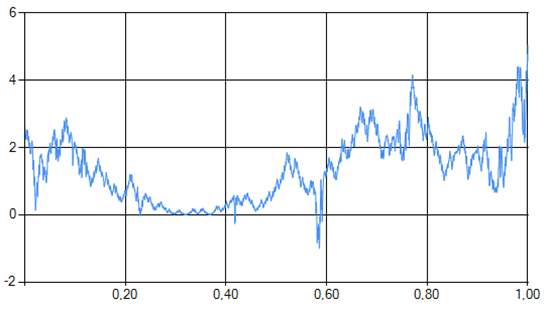
\includegraphics[width=0.8\textwidth]{fig1.png}
\caption{Heatmap of the function $R_{ps}(i)$ in the criteria space for algorithms with different machine learning models.} 
\label{fig:1}
\end{figure}

Fig. \ref{fig:1} shows the behavior of the characteristic $R_{ps}(i)$ in the criteria space for different models. Red points are related to the Pareto set, orange those to the class  where points are not effective ones. 

The color background displays the behavior of the penalty $R_{ps}(i)$ as a function of the criteria $f_1(y)$ and $f_2(y)$. Fig. \ref{fig:1}(a) shows the function $R_{ps}(i)$ for the method ML\_MGSA\_Dist. Fig. \ref{fig:1}(b,c,d) demonstrate $R_{ps}(i)$ for the different cases of the probabilistic models. Fig. \ref{fig:1}(b) corresponds to the model with linear kernel (ML\_MGSA\_Prob\_Linear), Fig. \ref{fig:1}(c) reflects results for the model with polynomial kernel (ML\_MGSA\_Prob\_Poly), and Fig. \ref{fig:1}(d) is related to RBF-based kernel (ML\_MGSA\_Prob\_RBF).
The number of trials carried out in each experiment is indicated in parentheses after the name of the method.

The figure shows that the penalty function with kernels other than linear describes the Pareto set well, but, may be, penalty is not sufficient to reduce the number of trials of the global search algorithm. Two modifications can be proposed to solve this problem.

First, when changing the optimization problem from set (\ref{eq:07}), a new weight calculation scheme for each of two classes of trial points is proposed. In this scheme, the weights of each class are calculated inversely proportional to the ratio of the number of all points to the number of points belonging to the Pareto set.

Second, the probabilities undergo the transformation
\begin{equation}
    \label{eq:18}
p'_i= \frac{ \log (p_i) - \log (p_{min})}{ \log (p_{max}) - \log (p_{min})} , 0 \leq i \leq k-1,
\end{equation}
where $p_i$ is a probability of the event that the point $x_i$ belongs to the Pareto set, $p_{min}$, $p_{max}$ are minimum and maximum values of such probabilities. After transformation the function $R_{ps}(i)$ is calculated, as earlier, as the average value of probabilities of events in which the points correspond to bounaries of the interval $(x_{i-1}, x_i)$ belong to the Pareto set.

Computational experiments were conducted for each method and each model in order to assess the effectiveness of using these techniques in the global search algorithm. Fig. \ref{fig:2} demonstrates the visualization of $R_{ps}(i)$ similar to Fig. \ref{fig:1}.
\begin{figure}
\centering
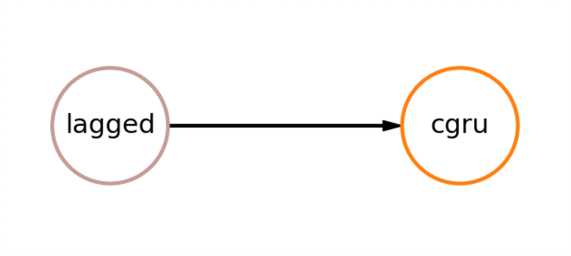
\includegraphics[width=0.8\textwidth]{fig2.png}
\caption{Heatmap of the function $R_{ps}(i)$ in the criteria space for algorithms with different techniques of building models after transformation (\ref{eq:18}).} 
\label{fig:2}
\end{figure}

Note that new penalty functions (see Fig. \ref{fig:2}(b,c,d)) describe better the Pareto set than functions built on the base of separating hyperplane. A detailed comparison of approaches to different computation of the characteristic (\ref{eq:16}) is given in Section \ref{sec:5}. 

\section{Results of computational experiments}
\label{sec:5}

Computations were conducted on the ``Lobachevsky'' supercomputer node (two Intel Sandy Bridge E5-2660 2.2 GHz processors and 64 Gb RAM) using the scikit-learn 0.24.2 library.
The proposed algorithms were implemented in Python in intelligent optimization framework iOpt \cite{iOpt_url}.

%Computations were performed with the support of the scikit-learn 0.24.2 framework.

%of the Nizhni Novgorod State University (operating system CentOS 7, control system SLURM).To obtain the executable program code the compilers Intel C++ 17.0.0 and python 3.9 were used.  and the optimization software iOpt \cite{iOpt_url}.

In the first experiment 100 bi-criterial MCO problems have been solved. As the partial criteria, the functions $f(y)$ from \cite{ML_MCO_2023} were taken,
\begin{equation}
    \label{eq:19}
		\begin{matrix}
		  f(y)= -(AB + CD)^{1/2} \\
			AB =(\sum_{i=1}^7{\sum_{j=1}^7{[A_{ij} a_{ij} (y_1,y_2) + B_{ij} b_{ij} (y_1,y_2)])}})^2 \\
			CD =(\sum_{i=1}^7{\sum_{j=1}^7{[C_{ij} a_{ij} (y_1,y_2) - D_{ij} b_{ij} (y_1,y_2)])}})^2 \\
			a_{ij} (y_1,y_2) = \sin(\pi i y_1) \sin(\pi j y_2), \\
			b_{ij} (y_1,y_2) = \cos(\pi i y_1) \cos(\pi j y_2),
		\end{matrix}
\end{equation}
where $0 \leq y_1, y_2 \leq 1$ and parameters $-1 \leq A_{ij},B_{ij},C_{ij},D_{ij} \leq 1$ are independent uniformly distributed random values.

Computational experiments for proposed techniques which utilize probabilities of belonging to the Pareto set can be divided into 3 groups.
\begin{enumerate}
	\item 	Experiments with the algorithm ML\_MGSA\_Prob (fixed weights);
	\item 	Solving MCO problems by the method ML\_MGSA\_Prob (Adjustive weights);
	\item 	Experiments with changing weights in the course of ML\_MGSA\_Prob running and transformed probabilities (\ref{eq:18})  (ML\_MGSA\_Prob (Norm Log)).
\end{enumerate}
	
In each series of experiments for these optimization algorithms, the coefficients $\alpha$ from (\ref{eq:16}) changed in the range $[0.1, 0.9]$. Comparison with the algorithm MGSA that does not use machine learning methods (i.e. with $\alpha = 0$ in the characteristic (\ref{eq:16})) and with the algorithm ML\_MGSA\_Dist taking into account the distance to the separating hyperplane was carried out. The comparison was made on the base of  the HV index characterizing quality of the obtained Pareto set approximation \cite{ML_MCO_2023,Evtushenko2014}. Further subsections include the results of only those calculations in which the $\alpha$ parameter provided the best quality of the solution found. Tables contain results of solving all the problems (\ref{eq:07}) with fixed accuracy $\varepsilon=0.01$ in the termination condition (\ref{eq:14}). Figures present results for a series of decreasing $\varepsilon$ which generates increasing numbers of trials.

\textbf{Experiments with fixed weights of two trial classes.} The first series of experiments is aimed at comparison the algorithm ML\_MGSA\_Prob (Fixed weights) with results of running for methods MGSA and ML\_MGSA\_Dist. 

The following parameters are indicated in Table \ref{tab:1}: the kernel of the SVM model (column 2), parameter $\alpha$ (column 3), average values of the HV-index (column 4), the average number of trials spent by the algorithm (column 5), and the coefficient of decreasing the number of trials compared to ML\_MGSA (column 6). The factors $r$ and $\varepsilon$ from (\ref{eq:10}) and (\ref{eq:14}) were the same for all the algorithms.

% Please add the following required packages to your document preamble:
% \usepackage{multirow}
% \usepackage{graphicx}
\begin{table}[ht]
\centering
\caption{Results of computational experiments}
\label{tab:1}
\resizebox{\textwidth}{!}{%
\begin{tabular}{cccccc}
\hline
\textbf{}                                                                  & \textbf{Model Kernel} & \textbf{$\alpha$} & \textbf{Avg. HV-index} & \textbf{Avg. iter.} & \textbf{Speedup} \\ \hline
ML\_MGSA                                                                   & -          & -    & 114.91  & 2269.82   & 1.00           \\ \hline
\multicolumn{6}{c}{\textbf{Experiments for the case of fixed weights}}                                                                \\ \hline
ML\_MGSA\_Dist                                                             & Linear     & 0.01 & 114.67  & 691.14    & \textbf{3.28}  \\
\multirow{3}{*}{ML\_MGSA\_Prob (Fixed weights)}                            & Linear     & 0.04 & 114.72  & 963.05    & 2.36           \\
                                                                           & Poly       & 0.07 & 114.73  & 871.82    & 2.60           \\
                                                                           & RBF        & 0.03 & 114.80  & 883.04    & 2.57           \\ \hline
\multicolumn{6}{c}{\textbf{Experiments for the case of adjusted weights}}                                                             \\ \hline
ML\_MGSA\_Dist                                                             & Linear     & 0.01 & 114.67  & 691.14    & \textbf{3.28}  \\
\multirow{3}{*}{ML\_MGSA\_Prob (Adj. weights)}                             & Linear     & 0.04 & 114.76  & 1018.03    & 2.23           \\
                                                                           & Poly       & 0.08 & 114.73  & 844.66    & 2.69           \\
                                                                           & RBF        & 0.03 & 114.76  & 796.74    & 2.85           \\ \hline
\multicolumn{6}{c}{\textbf{Experiments for the case of adjusted weights and logarithmic probabilities}}                                               \\ \hline
ML\_MGSA\_Dist                                                             & Linear     & 0.01 & 114.67  & 691.14    & \textbf{3.28}  \\
\multirow{3}{*}{ML\_MGSA\_Prob (Log Norm)}                                 & Linear     & 0.05 & 114.72  & 711.44    & 3.19           \\
                                                                           & Poly       & 0.04 & 114.79  & 854.82    & 2.66           \\
                                                                           & RBF        & 0.04 & 114.74  & 704.99    & 3.22           \\ \hline
\multicolumn{6}{c}{\textbf{Experiments with 4-criterial MCO problems}}                                                                \\ \hline
ML\_MGSA                                                                   & -          & -    & 7819.86 & 6046.4    & 1.00           \\ \hline
ML\_MGSA\_Dist                                                             & Linear     & 0.01 & 7751.43 & 1925.6    & 3.14           \\
\multirow{3}{*}{ML\_MGSA\_Prob (Log Norm)}                                 & Linear     & 0.08 & 7729.71 & 1760.5    & 3.43           \\
                                                                           & Poly       & 0.08 & 7796.20 & 4121.7    & 1.47           \\
                                                                           & RBF        & 0.08 & 7786.48 & 1364.6    & \textbf{4.43}  \\ \hline
\end{tabular}%
}
\end{table}

Fig. \ref{fig:3} shows the change of the average HV-index as a function of the number of trials.
\begin{figure}
\centering
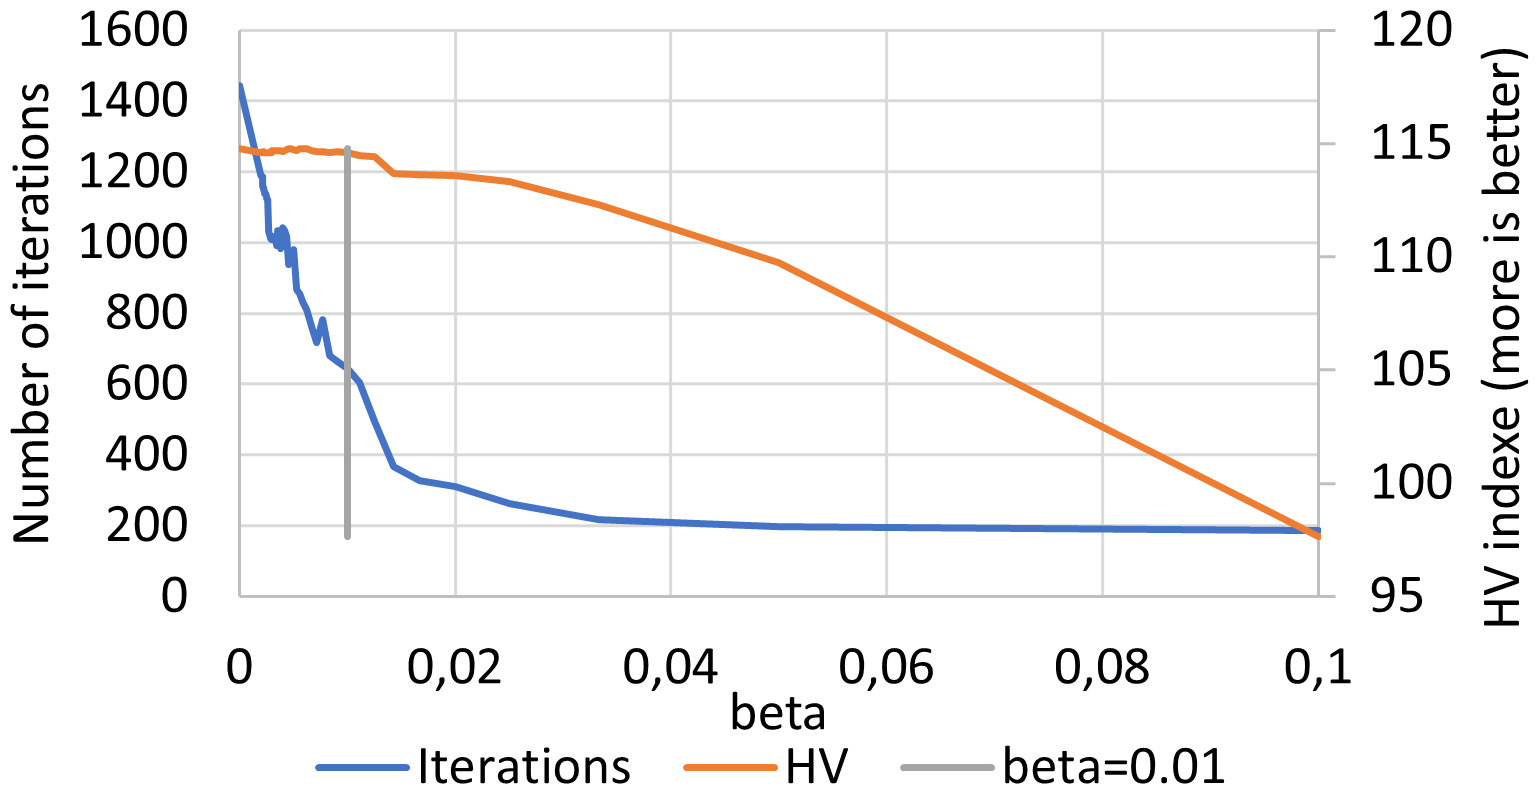
\includegraphics[width=0.8\textwidth]{fig3.png}
\caption{Comparison of HV-indices for the case of fixed weights.} 
\label{fig:3}
\end{figure}

Compared to MGSA, the other algorithms reduce significantly the number of iterations in conditions when HV-indices are similar. However, the iteration number when using the models with probabilities (see rows ``ML\_MGSA\_Prob (Fixed weights)'' of Table \ref{tab:1}) is greater than for the algorithm based on the separating hyperplane.

\textbf{Experiments with tuned weights in the course of optimization.} In this group of experiments the algorithm ML\_MGSA\_Prob (adj. weights) changed weights of trial classes before starting a new subproblem (\ref{eq:07}). Table \ref{tab:1} and Fig. \ref{fig:4} for these experiments are organized similarly to the first series of experiments.

\begin{figure}
\centering
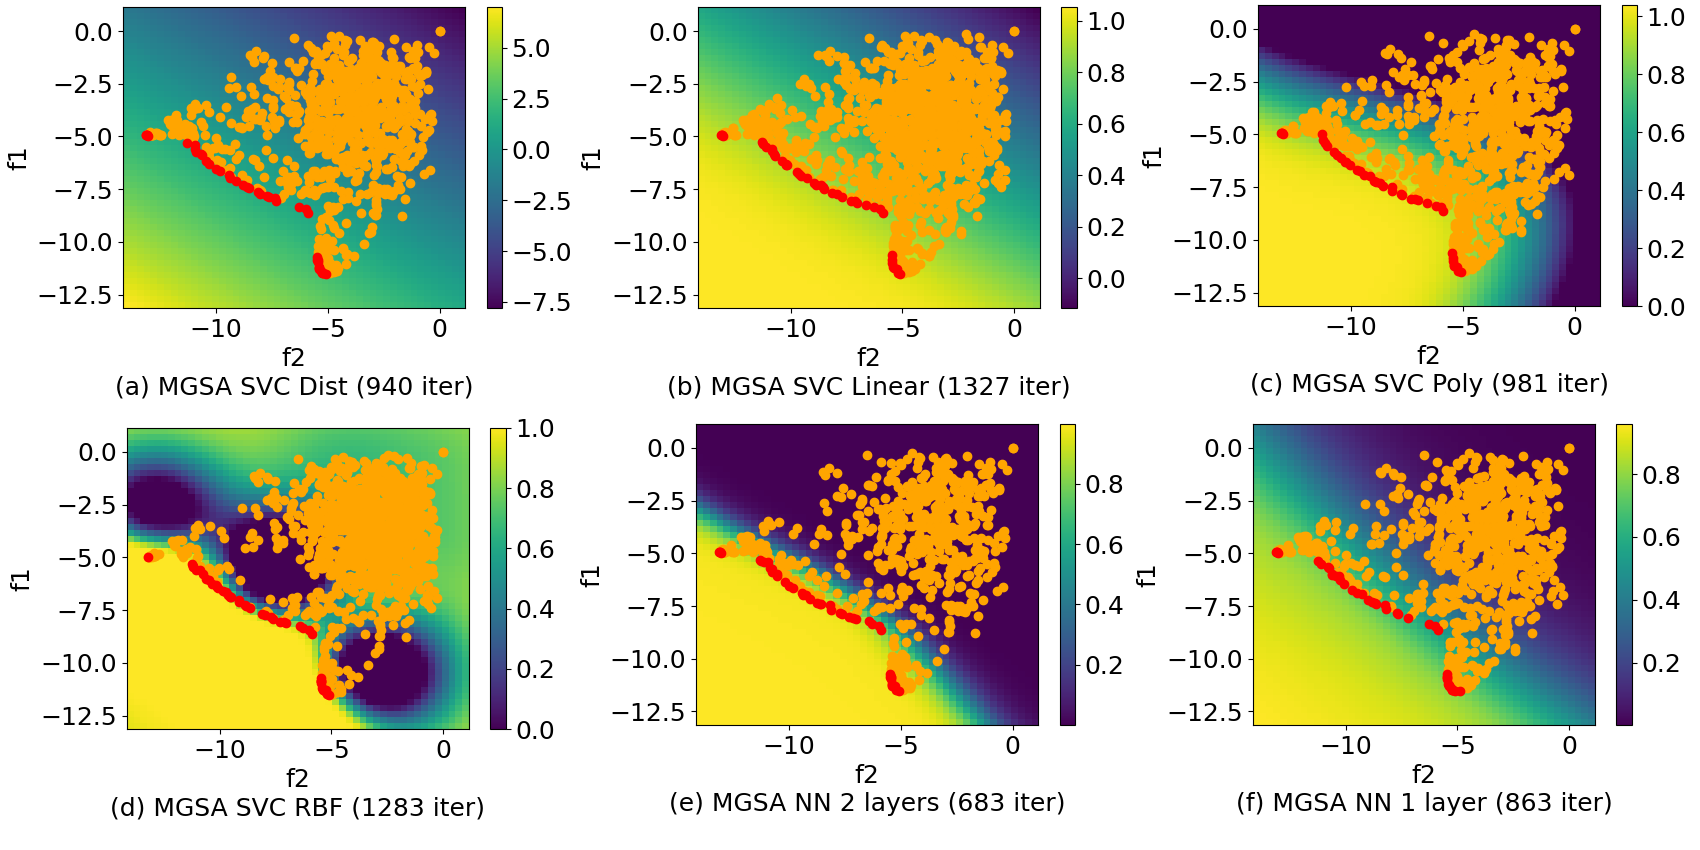
\includegraphics[width=0.8\textwidth]{fig4.png}
\caption{HV-indices comparison  in the case of adjusted weights} 
\label{fig:4}
\end{figure}

The presented data on methods using probabilities, as in the previous series of experiments, show significantly better results in the number of iterations compared to an algorithm without machine learning techniques. Nevertheless, from the results obtained, one cannot unequivocally say about a significant improvement or deterioration of these results compared to experiments in which the weights were set fixed.

\textbf{Experiments with adjusted weights and logarithmic probabilities.} In the third group of experiments, in addition to changing the weights during the algorithm’s running, the transformation (\ref{eq:18}) was used in techniques with probability calculation (methods ML\_MGSA\_Prob (Log Norm)). Table \ref{tab:1} and Fig. \ref{fig:5} are similar to those in the previous experiments.

\begin{figure}
\centering
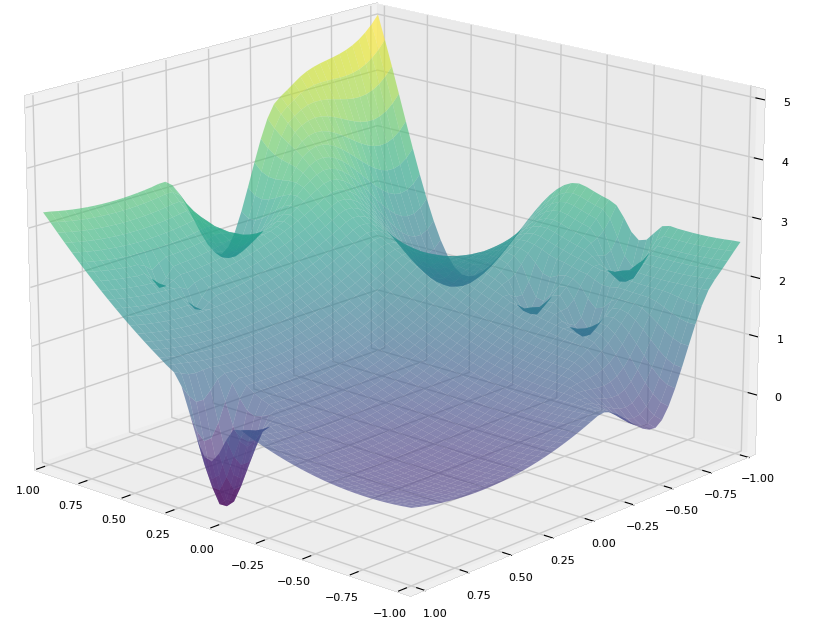
\includegraphics[width=0.8\textwidth]{fig5.png}
\caption{Comparison of  HV-indices for methods with probabilities (\ref{eq:18})} 
\label{fig:5}
\end{figure}

From the results of the experiment, the following conclusions can be drawn. Among the methods applying probabilistic techniques, the method with the transformation (\ref{eq:18}) demonstrates the best results. In the case of the SVM model with the linear kernel and with the RBF kernel, the results under increasing accuracy are comparable to the results obtained for ML\_MGSA\_Dist. At the same time, the techiques with probabilities enable changing easier the machine learning models. 

\textbf{Experiments with 4-criterial MCO problems.} In the last series of experiments, 10 MCO problems with 4 criteria were solved that form a Pareto set of complex structure. As in previous subsection, the functions of the family (\ref{eq:19}) were used as partial criteria. In the course of previous experiments, it was found that the closest result to ML\_MGSA\_Dist is given by the algorithm ML\_MGSA\_Prob (Log Norm) based on the technique (\ref{eq:18}). Taking into account this fact, we limited ourselves to comparing the results of these two algorithms. The results are presented in Table \ref{tab:1} and Fig. \ref{fig:6}

\begin{figure}
\centering
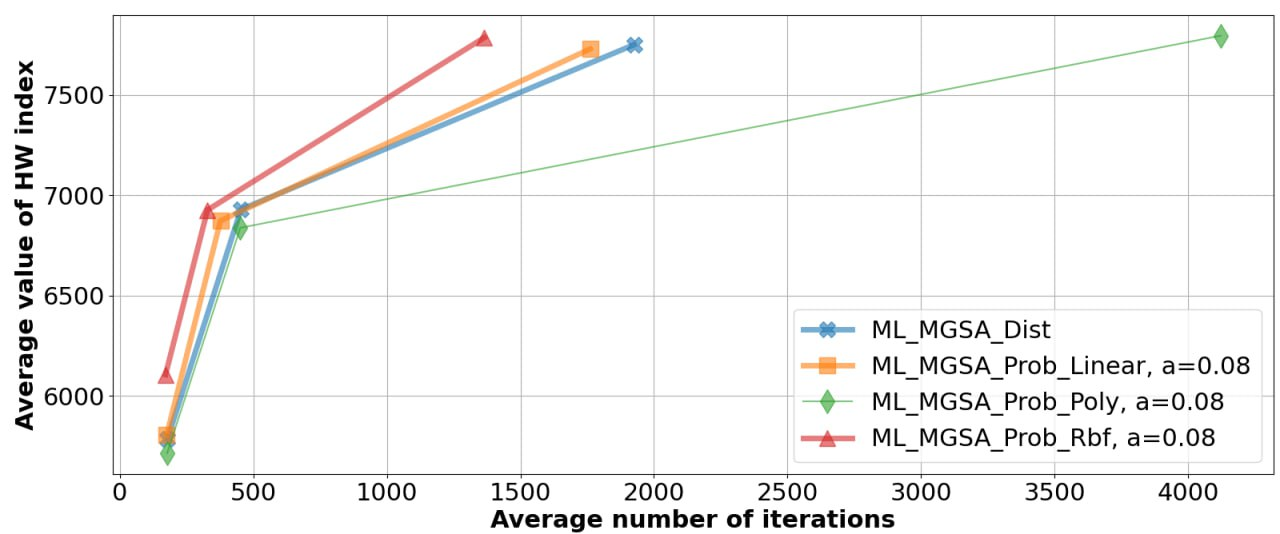
\includegraphics[width=0.8\textwidth]{Fig6.png}
\caption{Efficiency comparison in the 4-critarial case} 
\label{fig:6}
\end{figure}

The results of the experiments allow us to conclude that the method ML\_MGSA\_Prob (Log Norm) in this series of experiments can significantly reduce the number of trials with a similar value of HV-index compared to ML\_MGSA\_Dist. The best results were achieved using models with Linear and RBF kernels, while the latter model demonstrates better quality than the version of the algorithm with the technique \cite{ML_MCO_2023} based on distances to the hyperplane. 

\section{Conclusion}

The paper proposes a new modification of the global search algorithm focused on solving problems of multicriteria optimization. The algorithm in question is based on criteria scalarization and solving a series of multiextremal scalar problems. 

Acceleration of the algorithm (in terms of reducing the number of search trials required to evaluate the Pareto set) is achieved through the application of machine learning methods. Namely, when using the SVM method, trial points in the criteria space are classified (each point is/is not an efficient solution), on the basis of which a numerical estimate of the probability of belonging to the Pareto set is built. Polynomial and radial basis function kernels in SVM allows one to adequately approximate Pareto front of a complex structure. 

Solving several series of MCO problems with complex multiextremal criteria has demonstrated that the proposed approach to evaluating the set of efficient solutions is promising. Further research aims to develop the proposed approach by consideration of other machine learning models (in particular, artificial neural networks) to better classify trials and approximate the Pareto set.



%
% ---- Bibliography ----
%
% BibTeX users should specify bibliography style 'splncs04'.
% References will then be sorted and formatted in the correct style.
%
 \bibliographystyle{splncs04}
 \bibliography{bibliography}
%
%\begin{thebibliography}{8}
%\bibitem{ref_article1}
%Author, F.: Article title. Journal \textbf{2}(5), 99--110 (2016)
%
%\bibitem{ref_lncs1}
%Author, F., Author, S.: Title of a proceedings paper. In: Editor,
%F., Editor, S. (eds.) CONFERENCE 2016, LNCS, vol. 9999, pp. 1--13.
%Springer, Heidelberg (2016). \doi{10.10007/1234567890}
%
%\bibitem{ref_book1}
%Author, F., Author, S., Author, T.: Book title. 2nd edn. Publisher,
%Location (1999)
%
%\bibitem{ref_proc1}
%Author, A.-B.: Contribution title. In: 9th International Proceedings
%on Proceedings, pp. 1--2. Publisher, Location (2010)
%
%\bibitem{ref_url1}
%LNCS Homepage, \url{http://www.springer.com/lncs}, last accessed 2023/10/25
%\end{thebibliography}
\end{document}
